 \documentclass[conference]{IEEEtran}
\IEEEoverridecommandlockouts

\usepackage{cite}
\usepackage{amsmath,amssymb,amsfonts}
\usepackage{algorithmic}
\usepackage{graphicx}
\usepackage{textcomp}
\usepackage{xcolor}
\usepackage{graphics} % for pdf, bitmapped graphics files
\usepackage{epsfig} % for postscript graphics files
\usepackage{mathptmx} 
\usepackage{amsmath} % assumes amsmath package installed
\usepackage{amssymb}  % assumes amsmath package installed
\usepackage[utf8]{inputenc}
\usepackage[english]{babel} 
\usepackage{url}
\usepackage{hyperref}
\usepackage{graphicx}
\usepackage{color}
\usepackage{colortbl}
\usepackage{epstopdf}
\usepackage{filecontents}
\usepackage{comment}
\usepackage{amssymb}
\usepackage{verbatim}
\usepackage{indentfirst}
\usepackage{array}
\everymath{\displaystyle}
\usepackage{url}
\usepackage{enumitem} %For lists
\usepackage{array,tabularx}
\usepackage{textcomp}
\usepackage[T1]{fontenc}
\usepackage[utf8]{inputenc}
\usepackage{ifthen}
\usepackage{amsmath}
\usepackage{comment}
\usepackage{booktabs}
\usepackage{graphicx}
\usepackage[nolist]{acronym}

\def\oh{\tfrac{1}{2}}

\newcommand{\mat}[1]{\mathbf{#1}}
\def\H{^{\mathrm{H}}}
\def\T{^{\mathrm{T}}}

\usepackage[caption=false,font=footnotesize]{subfig}

\usepackage{tikz}
\usepackage{pgfplots}
\pgfplotsset{compat=1.10}

\usetikzlibrary{arrows,calc,positioning}

\def\BibTeX{{\rm B\kern-.05em{\sc i\kern-.025em b}\kern-.08em
    T\kern-.1667em\lower.7ex\hbox{E}\kern-.125emX}}
\begin{document}

\title{Coexisting Analysis of 5G Networks with ISDB-T System in TV White Spaces
%\title{Análise do Acesso Oportunista ao Espectro nas Faixas de UHF para Futuras Redes de Comunicações Móveis - 5G
%\title{Uma Análise de Coexistência entre Sistema ISDB-T de Radiodifusão e Futuras Redes de Comunicações Móveis - 5G
{\footnotesize \textsuperscript{}}
\thanks{}
}
%
\author{\IEEEauthorblockN{\textcolor{black}{Samuel de Souza Lima Moreira}}
\IEEEauthorblockA{\textcolor{black}{Francisco Martins Portelinha Júnior.}} 
\IEEEauthorblockN{\textcolor{black}{R\^omulo Mota Volpato}}
\IEEEauthorblockN{\textcolor{black}{Instituto Nacional de Telecomunicações - INATEL}}
\and
\IEEEauthorblockN{\textcolor{black}{Tales Cleber Pimenta}}
\IEEEauthorblockA{\textcolor{black}{Universidade Federal de Itajubá - UNIFEI}
}
}
\maketitle

\renewcommand\IEEEkeywordsname{Keywords}
\begin{IEEEkeywords}
ISDB-T, radiodifusão, 5G, GFDM, F-OFDM
\end{IEEEkeywords}

\pagenumbering{arabic} 
%//===========================================
%/ 01 Abstract:
%=========================================================
\begin{abstract}
O uso eficiente do espectro eletromagnético se torna cada vez mais necessário com o aumento de dispositivos conectados. Uma possível solução é utilização oportunista do espectro nas faixas de VHF e UHF, atualmente alocadas para transmissão de televisão. Portanto, torna-se necessário avaliar a operação conjunta entre sistemas de radiodifusão e sistemas de comunicação móvel. Este trabalho tem como proposta identificar, analisar e medir a interoperabilidade entre estes sistemas, verificando a viabilidade de coexistência de diferentes tipos serviços. Neste artigo, medições foram realizados entre duas fortes candidatas para a próxima geração celular, o GFDM e o F-OFDM, operando juntamento com o atual padrão de radiodifusão brasileiro. Os ensaios propostos demonstram a flexibilidade das formas de onda GFDM e F-OFDM sobre a atual forma de onda utilizada comercialmente o OFDM, possibilitando assim a utilização oportunista do espectro entre usuários licenciados e não licenciados.
\end{abstract}

% =========================================================
%\begin {abstract}
%Efficient use of the electromagnetic spectrum becomes increasingly necessary with the growth of connected %devices. One possible solution is opportunistic use of spectrum in the VHF and UHF bands currently allocated %for television broadcasting. Therefore, it is necessary to evaluate the joint operation between broadcasting %and mobile communication systems. This work aims to identify, analyze and measure the interoperability %between these systems, verifying the feasibility of coexistence of different types services. In this paper, %measurements were made between two strong candidates for the next generation of cell phone, GFDM and F-OFDM, %operating in conjunction with the current Brazilian broadcasting standard. The proposed tests demonstrate the %flexibility of the GFDM and F-OFDM waveforms over the current commercially used OFDM waveform, thus enabling %the opportunistic use of spectrum between licensed and unlicensed users.
%\end{abstract}

%/ 02 Introduction:
Section {Introduction}
%======================================================
Providing broadband access to the regions that do not have adequate coverage and meet the growing demand for traffic where the frequency resources are not, are crucial challenges for fifth generation of mobile 5G. One of the scenarios proposed for the next generation of mobile telephony is to enable mainly wireless broadband Internet access for rural areas, the WRAN vignettes (Texte {Wireless regional Area Network}) cite {IEEE_802_22}. The IEEE 802.22 standard deals with this challenge by proposing the exploration of idle channels, making use of network s of cognitive radios (Texte {RC}) cite {Wran}. Couple
%=====================================================
Weliston most of the electromagnetic spectrum has already been licensed by the regulatory agency, several measurements campaigns show that the rates of occupation of the electromagnetic spectrum are between 5% and 15% cite {IndoorWS} cite {White_Space _capacity }. With the analog TV shutdown process, a significant part of the spectrum in the VHF (very High Frequency) and UHF (Textif {Ultra High frequency}) range is being unoccupied cite {White_Space_Capacity, AnalogSwitchOff}. Parts that before Centrico localization for users products, license holders use the spectrum, are now availble for drug users. These gaps in the frequency spectrum are referred to as texte {blanks} cite {WSBook}. Couple
%=====================================================
In this context, the use of cognitive radios operating in the idle gaps of the spectrum is a solution to meet the needs observed, by allowing users to use the unlicensed tracks, optimizing the resources availble cite { WSBook}. However it is necessary to Absence that they do not cause El in the users products, spectrum holders. Couple
%=====================================================
In cite {GFDM}, the authors present a modulation technique with non-orthogonal carrier languages suitable for RC, because it allows the fragmented use of the spectrum and the control of emission to the range. This modulation technique is known as GFDM (textity(generalized Frequency Division multiplexing) and can be considered a generalization of the OFDM (Texti(orthogonal Frequency Division multiplexing)) cite {ref_OFDM}. The main feature that puts the GFDM as a promising transmission pattern for 5G is its flexibility to cite {heirOFDM}. Another technique proposed to decrease the emission is that of the range and decrease the emission of spurious is the use of the technique F-OFDM (Texte {Filtered-OFDM}) cite {FOFDM_hwawei} being a strong candidate to be adopted in was scenarios if for 5g. Couple
%=====================================================
Given the possibility of joint operation between TV systems and mobile communication systems in the UHF range, this work aims to Get a proposal to identify, analyse and measure interoperability between systems based on waveforms Proposals for the next generation cell operating in company channels in the TV range, and the current standard of Brazilian broadcasting the ISDB-T (TEXTT {Integrated Services Digital terrestrial Broadcasting). Through the analysis of the results, we evaluated the coexistence of legacy systems with the proposed waveforms for fifth generation of mobile communications. Couple
%====================================================
This article is organized as follows: In section II is presented a brief description of the waveforms studied, in section III describes the as system for conducting the experiments was assembled. In section IV, the procedures for conducting the tests are submitted and in section V the results of the interoperability test and coexistence of the different technologies studied. Finally, in section VI, the conclusions are elucidated.  Couple

\section{Introdução}
%======================================================
Prover acesso de banda larga para as regiões que não possuem cobertura adequada e atender à crescente demanda de tráfego onde os recursos de frequência são limitados, são desafios cruciais para quinta geração de celular o 5G. Um dos cenários propostos para a próxima geração da telefonia celular é viabilizar principalmente o acesso à Internet de banda larga sem fio para áreas rurais, as chamadas WRAN (\textit{Wireless regional area network}) \cite{IEEE_802_22}. O padrão IEEE 802.22 trata deste desafio propondo a exploração de canais ociosos, fazendo o uso de redes de rádios cognitivos (\textit{RC})\cite{wran}. \par
%=====================================================
Embora a maior parte do espectro eletromagnético já tenho sido licenciado pela agência reguladora, várias campanhas de medições realizadas mostram que as taxas de ocupação do espectro eletromagnético estão entre 5\% e 15\% \cite{IndoorWS}\cite{White_Space_Capacity}. Com o processo de desligamento da TV analógica, uma parte significativa do espectro na faixa de VHF (\textit{Very High Frequency}) e UHF (\textit{Ultra High Frequency}) está sendo desocupada \cite{White_Space_Capacity,AnalogSwitchOff}. Partes que antes estavam reservadas para usuários primários, detentores da licença de uso do espectro, agora estão disponíveis para usuários secundários. Estas lacunas no espectro de frequência são denominados de \textit{White Spaces} \cite{WSBook}. \par
%=====================================================
Neste contexto o emprego de rádios cognitivos operando nas lacunas ociosas do espectro é uma solução para atender as necessidades observadas, ao permitir que usuários secundários utilizem as faixas não licenciadas, otimizando os recursos disponíveis \cite{WSBook}. Entretanto é preciso garantir que os mesmos não causem interferências nos usuários primários, detentores do espectro. \par
%=====================================================
Em \cite{gfdm}, os autores apresentam uma técnica de modulação com múltiplas portadoras não ortogonais adequada para RC, pois permite o uso fragmentado do espectro e o controle da emissão fora da faixa. Esta técnica de modulação é conhecida como GFDM (\textit{Generalized Frequency Division Multiplexing}) e pode ser considerada uma generalização do OFDM (\textit{Orthogonal Frequency Division Multiplexing}) \cite{ref_OFDM}. A principal característica que coloca o GFDM como um padrão de transmissão promissor para o 5G é sua flexibilidade \cite{heirOFDM}. Uma outra técnica proposta para diminuir a emissão fora da faixa e diminuir a emissão de espúrios é a utilização da técnica F-OFDM (\textit{Filtered-OFDM}) \cite{fOFDM_hwawei} sendo uma forte candidata à ser adotada em alguns cenários previstos para o 5G. \par
%=====================================================
Dada a possibilidade de operação conjunta entre sistemas de TV e sistemas de comunicação móvel na faixa de UHF, este trabalho tem como objetivo apresentar uma proposta de para identificar, analisar e medir a interoperabilidade entre sistemas baseados em formas de ondas propostas para a próxima geração celular operando em canais ociosos na faixa de TV, e o atual padrão de radiodifusão brasileiro o ISDB-T (\textit{Integrated Services Digital Broadcasting Terrestrial}). Através da análise dos resultados, avaliou-se a coexistência de sistemas legados com as formas de onda propostas para quinta geração das comunicações móveis. \par
%====================================================
O presente artigo está organizado da seguinte maneira: Na Secção II é apresentado uma breve descrição das formas de ondas estudadas, na secção III descreve-se o como sistema para realização dos experimentos foi montado. Na secção IV são descritos os procedimentos para realização dos ensaios e na secção V os resultados dos teste de interoperabilidade e coexistência das diferentes tecnologias estudadas. Por fim na secção VI, as conclusões são elucidadas.\par

%/ 03 Waveforms:
\section{Waveforms} \label{sec:wave}
%=====================================================

O OFDM têm sido empregado como a interface padrão para a quarta geração celular e o atual padrão de transmissão terrestre \cite{ref_OFDM}. Contudo, o seu uso na camada física dificulta o acesso dinâmico ao espectro, devido à sua alta emissão de espúrios fora da faixa de interesse, o que torna necessário o uso de filtros para atender às normas impostas pelos órgãos de regulamentação. Portanto, para que o uso fragmentado do espectro possa ser eventualmente viável, o rádio transmissor deve reduzir as emissões fora da faixa minimizando as interferências nos canais adjacentes.\par
%======================================================
Os sistemas de comunicação atuais foram projetados para atingir a máxima capacidade de transmissão de dados possível, diferentemente dos requisitos almejados pela próxima geração de comunicação móvel. O 5G engloba diversos cenários, com características conflitantes, tornando um conceito mais amplo e complexo \cite{ref_pekka} e com a necessidade de uma maior flexibilidade na padronização de sua forma de onda. \par
%=======================================================

\subsection{GFDM}

A forma de onda GFDM pode ser descrita por sua flexibilidade em frequência e tempo, organizada em  $K$ sub-portadoras em frequência e $M$ sub-símbolos subsequentes no tempo, resultando em $N = KM$ versões diferentes de um pulso protótipo $g [n]$, cada um deslocado circularmente, tanto no domínio do tempo como no domínio da frequência, e modulado pelo símbolo de dados correspondente \cite{gfdm}, dado por \par

%=======================================================
\begin{equation}\label{eq:xn}
x[n] = \sum_{k=0}^{K-1}\sum_{m=0}^{M-1}d_{k,m}g\left[\left<n-mK\right>_N\right]{e}^{j2\pi\frac{k}{K}n},
\end{equation}
\nonident onde $d_{k,m}$ é o símbolo de dados carregado pela $k$-iésima sub-portadorea no $m$-ésimo sub-simbolo, $g[n]$ é o pulso protótipo, $\left<\cdot\right>_N$ é o operador modulo $N$ de $n=0,1,\ldots,N-1$. \par

%=======================================================
No receptor, admitindo que haja perfeita sincronia, e removido o prefixo cíclico (PC), o  sinal será equalizado no domínio da frequência, e pode então ser demodulado como \par

\begin{equation}
    \label{eq:dhat}
	\hat{d}=  \mathbf{B}_\textrm{ZF}\mathbf{y}_{\text{eq}}\\
\end{equation}
\noindent onde $\mathbf{y}_{\text{eq}}$ é o sinal recebido e equalizado e $\mathbf{B}_\textrm{ZF}$ é o processo de demodulação pela técnica \textit{zero-forcing} (ZF). \par

%======================================================

\subsubsection{W-GFDM}
%======================================================

O GFDM Janelado (W-GFDM) é uma variação que emprega uma janela no tempo para suavizar as transições entre os blocos GFDM. Nesta técnica o prefixo cíclico, com comprimento $NPC = NCH + NW$, onde onde NCH é o número de amostras da resposta ao impulso do canal e NW o tamanho da janela de transição, e o sufixo cíclico (CS) com $NCS = NW$, são utilizado somente uma vez por bloco.\par

%=======================================================
\subsection{F-OFDM}

A técnica f-OFDM vem sendo desenvolvida com a promessa de ser uma solução simples para o problema de emissão fora da faixa do OFDM. Neste esquema, dados destinados a cada usuário são tratados de maneira independente, correspondendo ao sinal que será transmitido em cada uma das $L$ sub-bandas. Para o sinal de cada sub-banda, os \textit{bits} são mapeados em símbolos de dado e agrupados em $K_{l}$ símbolos, em que $K$ é o número de subportadoras da $l$-ésima sub-banda, sobre os quais será computada cada uma das $L$ IFFT. É, então, adicionado um PC de tamanho $N_{\text{PC}_{l}}$ e o sinal resultante é filtrado, por sub-banda, por um filtro $g_{l}[n]$. \par
%=======================================================

Em \cite{fOFDM_hwawei} é proposto um sistema f-OFDM em que o transmissor gera seu sinal OFDM empregando um grupo de $K_{l}$ subportadoras consecutivas ao longo de $M$ símbolos OFDM consecutivos. O sinal transmitido por cada terminal móvel é dado por \par

%==================================================
\begin{equation}
x_{\text{f}}[n] = \sum_{m = 0}^{M-1}x_{m}(n - m(K_{l} + N_{\text{PC}_{l}}))
\end{equation}
%==================================================
em que
%==================================================
\begin{equation}
x_{m}[n] = \sum_{k = k^{'}}^{k^{'} + K_{l} - 1}d_{m,k}\exp\bigg(j2\pi \frac{k}{K_{l}}n\bigg)
\hspace{0.2cm}\textrm{para}\hspace{0.5cm} -N_{\text{PC}_{l}} \leq n \leq N.
\end{equation}
%==================================================

O sinal f-OFDM é então obtido através da filtragem do sinal $x_{f}[n]$ através filtro protótipo apropriado $g_{l}[n]$, que pode ser descrito pelo processo de convolução, desta maneira teremos, \par
%==================================================

\begin{equation}
\centering
\bar{x}_{\text{f}}[n] = x_{\text{f}}[n] * g_{l}[n]
\end{equation}

%=======================================================
\nonident onde $\bar{x_{\text{f}}[n]}$ é o sinal da $l$-ésima sub-banda. O dimensionamento do filtro protótipo tem de ser apropriado para mitigar as emissões fora da faixa. No receptor na entrada da estação rádio base, o sinal recebido dos sinal dos $u$-ésimos usuários é dado por \cite{fOFDM_hwawei}, \par
% Veja se concorda com essa frase e se ficou boa!!!

%=======================================================
\begin{equation} \label{eq:received}
y[n] = \sum_{u = 0}^{U} \bar{x}_{\text{u}}[n] * h_{u}[n] + w[n]
\end{equation}

%=======================================================
onde $U$ é o número de terminais móveis, $\bar{x}_{\text{u}}[n]$ é o sinal do $u$-ésimo usuário, $h_{u}[n]$ é a resposta impulsiva do canal do $u$-ésimo canal e $w[n]$ é ruído aditivo gaussiano branco (AWGN). Após a recepção, o sinal é passado primeiramente por um filtro casado $g_{l}[n]^*$, haverá a remoção do prefixo cíclico, transformação do sinal do domínio do tempo para frequência, equalização e por fim a demodulação dos mesmos. \par

%/ 04 System Setup:
\section {System Setup and Development}
Para realizar os ensaios de convivência elaborou-se um arranjo de equipamentos, conforme ilustra a Figura
%To perform the coexistence tests, an arrangement of equipment was elaborated, as illustrated by figure
\ref{fig:SetupMedidas}. \par
%=========================================================
%=========================================================
O sistema foi operado através de um controlador embarcado responsável por rodar e gerenciar a aplicação desenvolvida. Para geração do \textit{Transport} \textit{Stream} (TS) utilizou-se um adaptador ASI (\textit{Asynchronous serial interface}) ligado a um modulador de TV digital (TVD) no padrão ISDB-T. Os sinais 5G foram transmitidos por um rádio definido por \textit{software} (RDS).\par

%The system was operated through an embedded controller responsible for rotating and managing the developed application. For generation of Texti{transport} Texti{stream} (TS) an ASI adapter (Texti{asynchronous serial Interface}) was used connected to a digital TV modulator (TVD) in the ISDB-T standard. 5G signals were transmitted by a radio set by texti{software} (RDS) .par

%==========================================================

O conjunto de sinais interferido e interferente foram agrupados, em meio confinado, utilizando um combinador de RF (Radiofrequência). Por fim o arranjo foi ligado aos receptores TVD. A observação da imagem foi realizada em uma televisão de uso doméstico. A conferência dos sinais no espectro eletromagnético e as medidas de potência de canal foram realizadas com um analisador digital de sinais. \par

%The set of interfered and interferent signals were grouped in a confined medium using an RF combiner (radiofrequency). Finally, the arrangement was connected to the TVD receptors. The observation of the image was performed on a home television. The Conference of Signals in the electromagnetic spectrum and the measurements of channel power were performed with a digital signal analyzer. par

%==========================================================

\begin{figure}[h!]
    \centering
    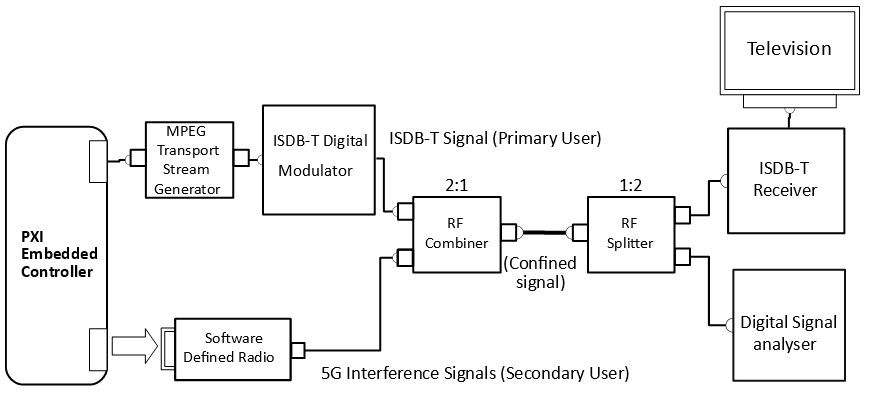
\includegraphics[width=0.45\textwidth]{Figures/setup_full_v3.jpg}
    \caption{Measurement setup proposed for coexistance procedures}
    \label{fig:SetupMedidas}
\end{figure}

%==========================================================

\subsection {Desenvolvimento da aplicação}
%==========================================================

A aplicação desenvolvida é composta por uma sessão de usuário e outra para interface com o rádio, como pode ser visto na Figura \ref{fig:DiagramaLabview}. O sistema gera um vetor de amostras em banda base\footnote{Referência de códigos para geração dos sinais 5G: \url{https://github.com/kit-cel/gr-gfdm}}, de acordo com seleção do usuário, modulado em uma das formas onda para a 5G descritas na secção \ref{sec:wave}. Uma vez que a configuração é feita, as amostras são então transferidas para o RDS. \par


%The application developed is composed of one user session and another for interface with the radio, as can be seen in Figure ref{fig: DiagramaLabview}. The system generates a vector of samples in band Basefootnote {code reference for generating 5G signals: url{https:/github.com/kit-cel/gr-gfdm}}, according to user selection, modulated in one of the waveforms for 5G described in section ref{sec: Wave }. Once the configuration is done, the samples are then transferred to the RDS. par


%==========================================================

\begin{figure}[h!]
    \centering
    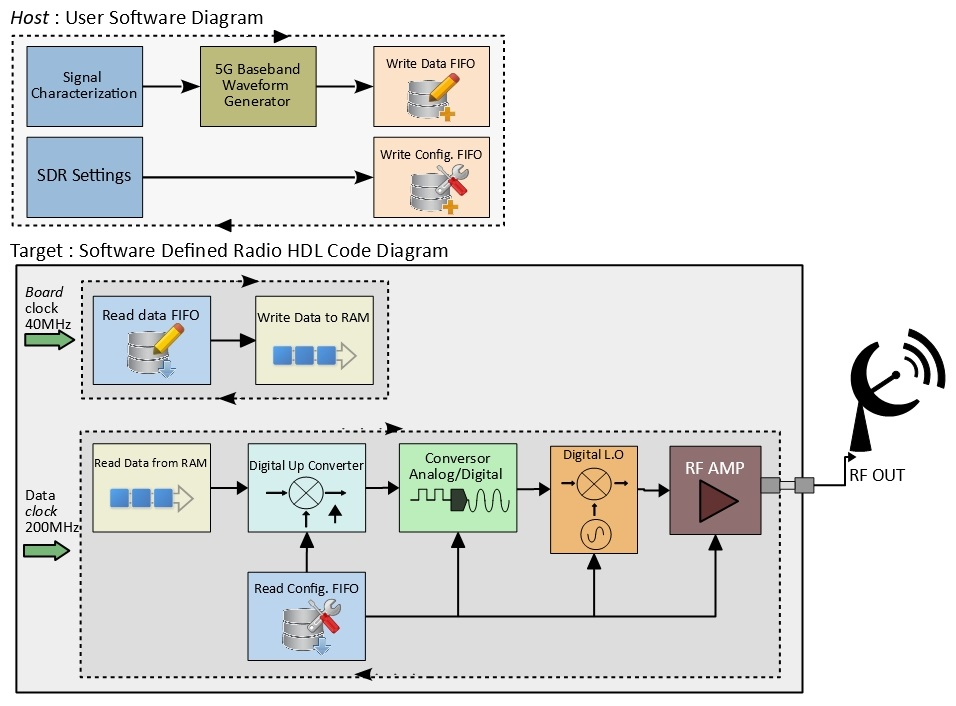
\includegraphics[width=0.45\textwidth]{Figures/Diagrama_Labview_full_v3.jpg}
    \caption{5G Waveform generator system block diagram}
    \label{fig:DiagramaLabview}
\end{figure}

%==========================================================

The data is written to a RAM and repeated sequentially until a new vector of samples is generated. The stream is converted to an intermediate frequency and then delivered to the analog digital converter. Finally the sequence is translated to channel frequency, and the RF transmission is performed. \par
%==========================================================



%/ 05 Test Procedures:
\section {Signal Characterization and Test Procedures}

In domestic ISDB-T receivers It is not commonly possible to perform bit error rate measures. Thus, new methods were proposed by ITU (Texti{international Telecommunications Union}) to establish the protection relationship, and to ensure the quality of service. The criterion chosen in this study to determine the point of failure was based on the recommendation ITU-R BT. 1368-12 cite{ITU_BT_1368}, where the protection relationship is determined subjectively through the evaluation of image quality. par
%=========================================================

The application of the method was performed by varying the level of the interfering signal, while the image received was observed. The level of the primary service was kept constant, at a pre-established value, while the level of the interfering signal was increased to the point where it became noticeably noticeable constant errors or image freezing, regardless of the visual acuity of the Observer. It was used, as recommended, that the limit condition occurs when there are no errors in the image in the first 20 seconds of observation. par
%=========================================================

The tests performed consider that the channels are spaced at 428.571 KHz, as illustrated in Figure ref{fig: ISDB_channel_Spacing} cite{ARIB_STD_B31} and cite{NBR_15601}. To measure the channel power was adopted 6MHz and 18MHz of integration bandwidth, with resolution of 100KHz. \par

\begin{figure}[h!]
    \centering
    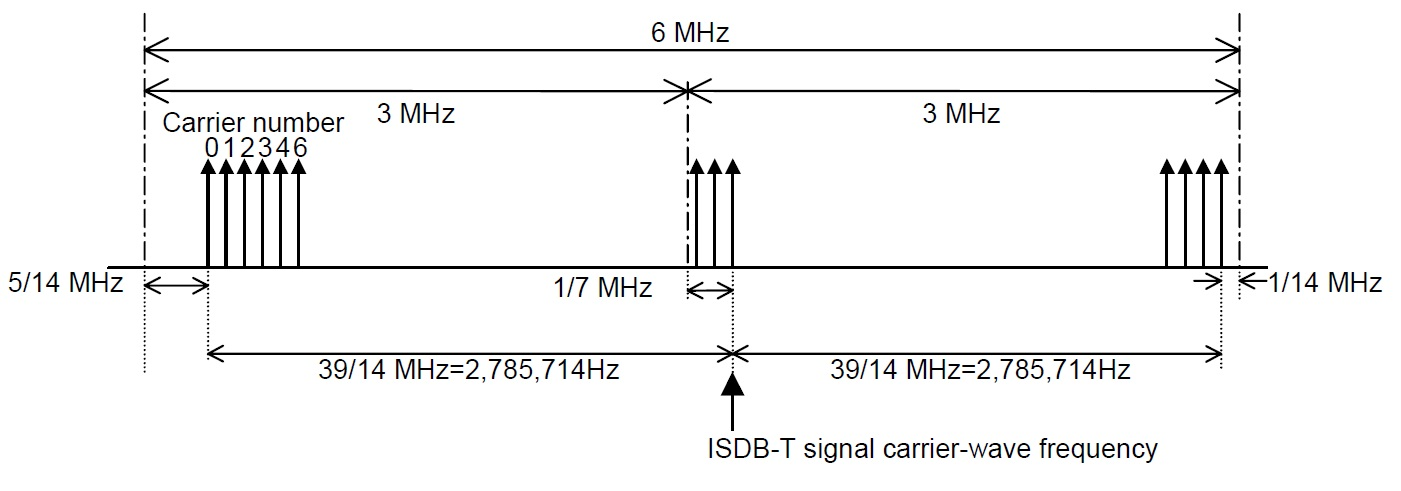
\includegraphics[width=0.45\textwidth]{Figures/Arib_ISDB_T_channel_Spacing}
    \caption{ISDB-T channel spacing}
    \label{fig:ISDB_channel_Spacing}
\end{figure}

%=========================================================
\subsection{ISDB-T Signal characterization}
%=========================================================

The characterization of the digital TV signal used in the tests was performed according to the parameters presented in table ~ ref{tab: table_ISDBT}. par
%=========================================================

\begin{table}[h!]
	\begin{center}
		\centering
		\caption{Caracterização do sinal de ISDB-T usado nos testes laboratoriais.}
		\label{tab:table_ISDBT}
		\begin{tabular}{|l|c|c|c|}
			\hline
			\textbf{Camada} & \textbf{A} & \textbf{B} & \textbf{C}\\
			\hline
			Número de segmentos & 13 & - & -\\
			\hline
			Modulação & 64QAM & - & -\\
			\hline
			FEC & 3/4 & - & -\\
			\hline
			Entrelaçamento no Tempo & 2 & - & -\\
			\hline
			Largura de banda &\multicolumn{3}{c|}{5,572421MHz}\\
			\hline
			Recepção Parcial &\multicolumn{3}{c|}{Não}\\
			\hline
			Modo &\multicolumn{3}{c|}{\textit{Mode} 3}\\
			\hline
		    Intervalo de Guarda &\multicolumn{3}{c|}{1/8}\\
			\hline
		\end{tabular}
	\end{center}
\end{table}
%=========================================================

\subsection {Ajuste do limiar de recepção dos receptores ISDB-T}
%=========================================================

The receiving threshold expresses the level in dBm under which the receiving test must operate throughout the tests. The following procedures were adopted to determine the receiving threshold cite{LTE_ISDBT}. par


\begin{enumerate}[label=(\alph*)]
    %a
    \item Aplicou-se um vídeo TS de referencia, na respectiva entrada do modulador.
    %b
    \item Ajustou-se o sinal de TVD para o canal 32 UHF, inicialmente com o nível de -70 dBm e modulação 64QAM, caracterizado conforme descrito na tabela \ref{tab:table_ISDBT}. Conferiu-se se o video estava sendo exibido sem falhas pelo receptor em teste.
    %c
	\item O nível do sinal de TVD foi reduzido até que houvesse falha visível e constante na imagem, independente da acuidade visual do observador. Observou-se a estabilização da qualidade da imagem por pelo menos 20s, conforme determina \cite{ITU_BT_1368}.
    %d
    \item O nível foi conferido utilizando analisador digital se sinais, no modo de medição de potência de canal.Partindo do limiar de visibilidade, o nível  do sinal foi aumentado em 3 dB.
    %e
    \item Os itens de (a) a (e) foram então repetidos para todos os receptores.
\end{enumerate}

%=========================================================
%\begin{table}[h!]
%	\begin{center}
%		\centering
%		\caption{Nível de operação dos receptores ISDB-T.}
%		\label{tab:Receptores}
%		\begin{tabular}{|l|c|c|c|c|}
%			\hline
%			\textbf{Receptor} & \textbf{RX1} & \textbf{RX2} & \textbf{RX3} & \textbf{RX4}\\
%			\hline
%			Nível (dBm/6MHz)&-75,7 & -75,2 & -79,7 & -75,1\\
%			\hline
%			Nível (dBm/18MHz)&-75,2 & -73,7 & -77,9 & -73,8\\
%			\hline
%		\end{tabular}
%	\end{center}
%\end{table}
%=========================================================

\subsection{Interferência em canal adjacente}

The objective of this experiment is to establish the harmful interference point for operation in adjacent channels, by determining the saturation threshold (the $ _{th} $) that expresses the power in dBm from the TVD receiver loses the ability to discriminate The interferent signal of the desired. The following steps were performed to perform this assay, par  
%=========================================================

\begin{enumerate}[label=(\alph*)]
    \item   O sinal ISDB-T caracterizado anteriormente foi ligado ao arranjo de medidas.
    \item 	Aplicou-se inicialmente um sinal interferente modulado com a tecnologia OFDM operando no canal adjacente inferior ($N$-1).  
    \item 	A potência do sinal interferente foi aumentada em passos de 0,5dB até que a imagem analisada apresentasse erros constantes.
    \item 	Ao atingir a condição limite, a potência do canal adjacente foi medida.
    \item 	Repetiu-se os procedimentos (a) até (d) variando entre as tecnologias GFDM, W-GFDM e F-OFDM.
    \item 	Por fim, repetiu-se os itens (a) até (e) operando agora no canal adjacente superior ($N$+1).
\end{enumerate}
%=========================================================

The characterization used is shown in the table ref{tab: table_ADJ_01}.
%=========================================================

\begin{table}[h!]
	\begin{center}
		\centering
		\caption{Configuração dos sinais interferente para teste de interferência  em canais adjacentes.}
		\label{tab:table_ADJ_01}
		\begin{tabular}{|l|c|c|c|c|}
			\hline
			\textbf{} & \textbf{OFDM} & \textbf{GFDM} & \textbf{W-GFDM} & \textbf{F-OFDM}\\
			\hline
			$M$ & 1 & 3 & 3 & 1\\
			\hline
			$K$ &\multicolumn{4}{c|}{512}\\
			\hline
			$KoffS$ &\multicolumn{4}{c|}{128}\\
			\hline
			$KoffC$ &\multicolumn{4}{c|}{0}\\
			\hline
			$nCP$ &\multicolumn{4}{c|}{64}\\
			\hline
			$nCS$ & 0 & 0 & 50 & 0\\
			\hline
			$nW$ & 0 & 0 & 50 & 0\\
			\hline
		\end{tabular}
	\end{center}
\end{table}
%=========================================================

\newenvironment{conditions*}
  {\par\vspace{\abovedisplayskip}\noindent
   \tabularx{\columnwidth}{>{$}l<{$} @{${}={}$} >{\raggedright\arraybackslash}X}}
  {\endtabularx\par\vspace{\belowdisplayskip}}

Onde:

\begin{conditions*}

M & Sub símbolos \\
K & Total de portadoras\\   
KoffS & Portadoras desligadas lateralmente\\
KoffC & Portadoras desligadas ao centro\\
nCp & Amostras de prefixo cíclico\\
nCp & Amostras de sufixo cíclico\\
nW  & Amostras de janela\\
\end{conditions*}

%\begin{conditions*}
%M & N\textsuperscript{\underline{o}} de sub símbolos \\
%K & N\textsuperscript{\underline{o}} total de portadoras\\   
%KoffS & N\textsuperscript{\underline{o}} de portadoras desligadas lateralmente\\
%KoffC & N\textsuperscript{\underline{o}} de portadoras desligadas no centro do sinal\\
%nCp & N\textsuperscript{\underline{o}} de amostras de prefixo-cíclico\\
%nW  & N\textsuperscript{\underline{o}} de amostras da janela\\
%\end{conditions*}

\subsection{Interferência com sinal operando canais associados e portadoras desligadas}
%=========================================================

One of the features of 5G waveforms designed for this assay is the ability to disconnect the central carriers, thus allowing the association of multiple idle channels. The proposed experiment intends to evaluate the ability of 5G waveforms to occupy multiple channels, without generating interferences in the existing primary services. par% An example of this scenario is illustrated in Figure ref{fig: setupLabview2}. 
The same procedures of the previous experiment were adopted, with the difference that to perform the power measurements, the ISDB-T signal was first disconnected. The characterization of this procedure is described in the table ref{tab: table_ADJ_02}. par
%=========================================================

\begin{table}[h!]
	\begin{center}
		\centering
		\caption{Caracterização para ensaio em múltiplos canais adjacentes.}
		\label{tab:table_ADJ_02}
		\begin{tabular}{|l|c|c|c|c|}
			\hline
			\textbf{} & \textbf{OFDM} & \textbf{GFDM} & \textbf{W-GFDM} & \textbf{F-OFDM}\\
			\hline
			$M$ & 1 & 3 & 3 & 1\\
			\hline
			$K$ &\multicolumn{4}{c|}{512}\\
			\hline
			$KoffS$ &\multicolumn{4}{c|}{104}\\ 
			\hline
			$KoffC$ &\multicolumn{4}{c|}{152}\\ 
			\hline
			$nCP$ & 64 & 50 & 50 & 64\\
			\hline
			$nCS$ & 0 & 0 & 50 & 0\\
			\hline
			$nW$ & 0 & 0 & 50 & 0\\
			\hline
		\end{tabular}
	\end{center}
\end{table}

%\begin{figure}[h!]
%    \centering
%    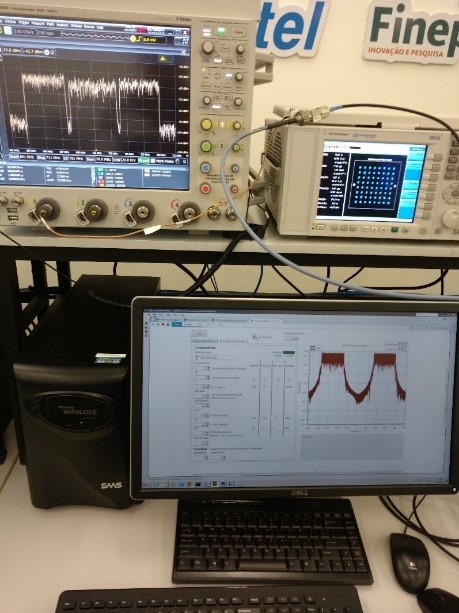
\includegraphics[width=0.25\textwidth]{Figures/setup_CRR.jpg}
%    \caption{Sinal 5G com canais associados e portadoras desligadas.}
%    \label{fig:setupLabview2}
%\end{figure}

%/ 06 Results:
\section{Measurements Results}

Initially, the operating levels of each of the evaluated receptors were collected, presented in the table ref{tab: receivers}, through the determination of the reception threshold as described in the previous section. These measures were used as a reference for comparing the results of the. 

% Tabela receptores
%=========================================================
\begin{table}[h!]
	\begin{center}
		\centering
		\caption{ISDB-T Receivers operational level}
		\label{tab:Receptores}
		\begin{tabular}{|l|c|c|c|c|}
			\hline
			\textbf{Receptor} & \textbf{RX1} & \textbf{RX2} & \textbf{RX3} & \textbf{RX4}\\
			\hline
			Power Level (dBm/6MHz)&-75,7 & -75,2 & -79,7 & -75,1\\
			\hline
			Power Level (dBm/18MHz)&-75,2 & -73,7 & -77,9 & -73,8\\
			\hline
		\end{tabular}
	\end{center}
\end{table}
%=========================================================

%Limiar de saturação (Oth) para interferência de canal adjacente
\begin{table*}[t!]
	\begin{center}
		\centering
		\caption{ $O_{th}$ para teste de interferência em canais adjacentes}
		\label{tab:Resultados_ADJ01}
		\begin{tabular}{|c|c|c|c|c|c|c|c|c|}
			\hline
			\textbf{Receptores}&\multicolumn{2}{c|}{\textbf{RX1}}&\multicolumn{2}{c|}{\textbf{RX2}}&\multicolumn{2}{c|}{\textbf{RX3}}&\multicolumn{2}{c|}{\textbf{RX4}}\\
			\hline
			\textbf{Canal UHF}&\textbf{31}&\textbf{33}&\textbf{31}&\textbf{33}&\textbf{31}&\textbf{33}&\textbf{31}&\textbf{33}\\
			\hline
			\textbf{OFDM (dBm/6MHz)} &-53,4&-53,1&-54,4&-53,6&-53,2&-53,6&-53,6&-53,4\\
			\hline
			\textbf{GFDM (dBm/6MHz)} &-47,3&-47,4&-50,1&-50,2&-49,3&-49,2&-49,2&-49,3\\
			\hline
			\textbf{W-GFDM (dBm/6MHz)}&-38,0&-39,8&-41,2&-41,2&-42,8&-39,7&-41,2&-41,1\\
			\hline
			\textbf{F-OFDM (dBm/6MHz)}&-38,5&-38,6&-41,7&-40,3&-43,5&-39,7&-41,2&-40,2\\
			\hline
		\end{tabular}
	\end{center}
\end{table*}
%=========================================================

\begin{figure}[h]
    \centering
    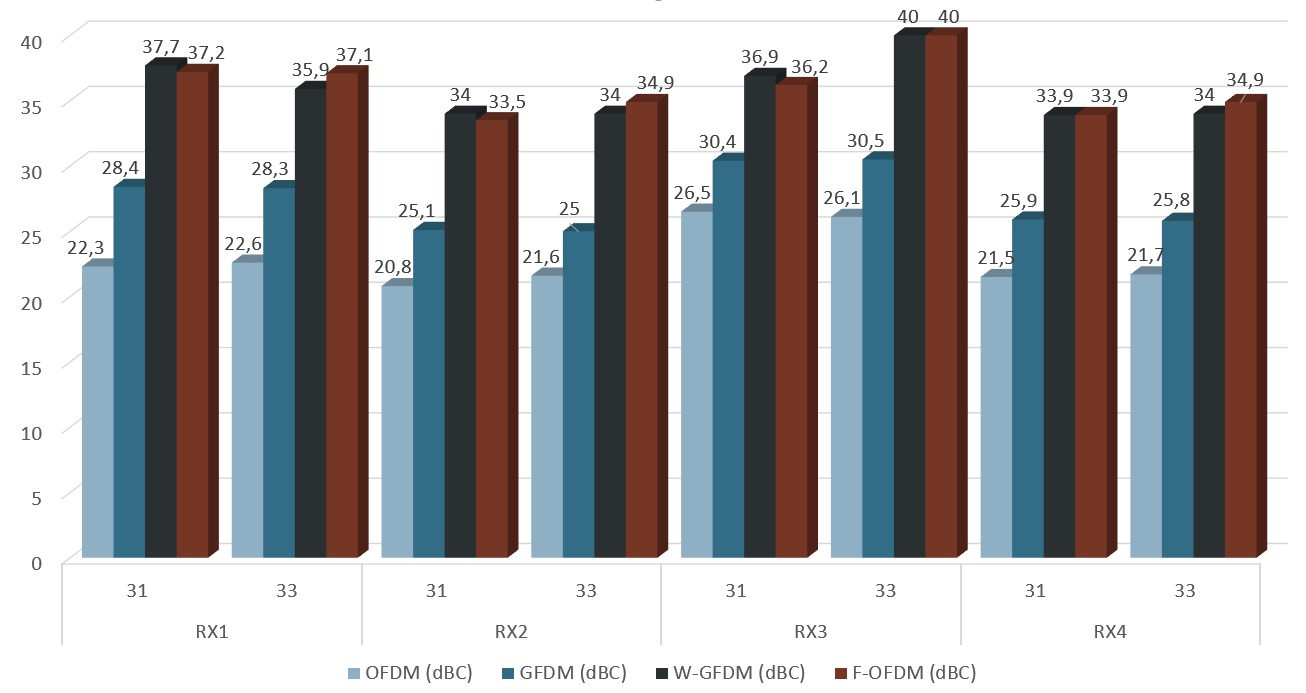
\includegraphics[width=0.48\textwidth]{Figures/result_01.jpg}
    \caption{$O_{th}$ Comparrisson with ISDB-T operational level for adjacent channel test (dBc)}
    \label{fig:result_01}
\end{figure}

%=========================================================

%Limiar de saturação (Oth) para interferência com sinal ocupando multiplos canais
\begin{table}[h!]
	\begin{center}
		\centering
		\caption{$O_{th}$ medido em ensaio de interferência com sinais ocupando múltiplos canais}
		\label{tab:Resultados_ADJ02}
		\begin{tabular}{|c|c|c|c|c|}
			\hline
		    \textbf{}&\textbf{RX1} & \textbf{RX2} & \textbf{RX3} & \textbf{RX4}\\
			\hline
			OFDM (dBm/18MHz) &-65,25&-65,2&-68,2&-66,8\\
			\hline
			GFDM (dBm/18MHz) &-59,2&-60,7&-63,7&-63,0\\ 
			\hline
			W-GFDM (dBm/18MHz) &-42,2&-41,9&-43,9&-43,2\\
			\hline
			F-OFDM (dBm/18MHz) &-65,3 &-65,2&-68,3&-66,9\\
			\hline
		\end{tabular}
	\end{center}
\end{table}

%=========================================================

\begin{figure}[h]
    \centering
    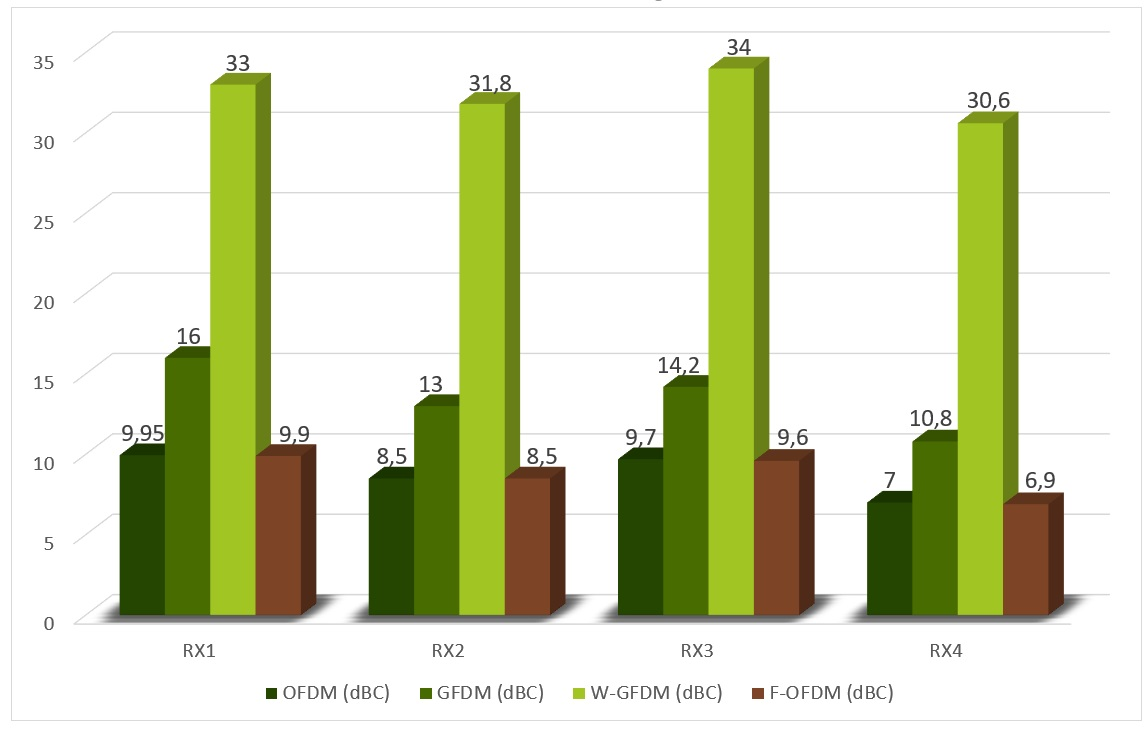
\includegraphics[width=0.48\textwidth]{Figures/result_02.jpg}
    \caption{$O_{th}$ Comparrisson with ISDB-T Operational Level for multiple channel test (dBc)}
    \label{fig:result_02}
\end{figure}

%=========================================================

Comparing the measurements of $O _{th} $ shown in the table ref{tab: Resultados_ADJ01} for the interference test on adjacent channels it is verified that the F-OFDM and W-GFDM transmission techniques caused harmful interference operating at the level of Higher power in all tested equipment. Making the relationship with the operating threshold, as shown in Figure ~ ref{fig: result_01} It is noted that in this experiment there was no significant difference between these technologies. par

%=========================================================

In the experiment with signals operating in multiple channels and disconnected carriers, as shown in table ref{tab: Resultados_ADJ02}, once again it was found that the W-GFDM transmission technique interfered with the primary service, with the highest level. In this scenario the $O _th $ for the modulated signal in F-OFDM practically showed no advantages when compared to OFDM, as can be seen in Figure ~ ref{fig: result_02}. We believe that this result is due to the type of prototype filter used in base-band signal generation and deeper studies should be done to mitigate this problem. par
%=========================================================

The results of the measurements indicated that out-of-band emissions for the modulations proposed for 5G are lower when compared to the OFDM technique. Figure ~ ref{fig: Waveforms} illustrates this situation, where you can see the difference between the technologies by measuring the spectral densities of power. The more efficient use of the PC gives the W-GFDM greater spectral efficiency and energy savings when compared to the other modulations analyzed. This feature is important in the WRAN scenario, where the major delays of channel paths require long cyclical prefixes cite{IEEE_802_22}. Therefore, this is quite promising for operations in texti{white spaces}. par
%=========================================================

\begin{figure}[h]
    \centering
    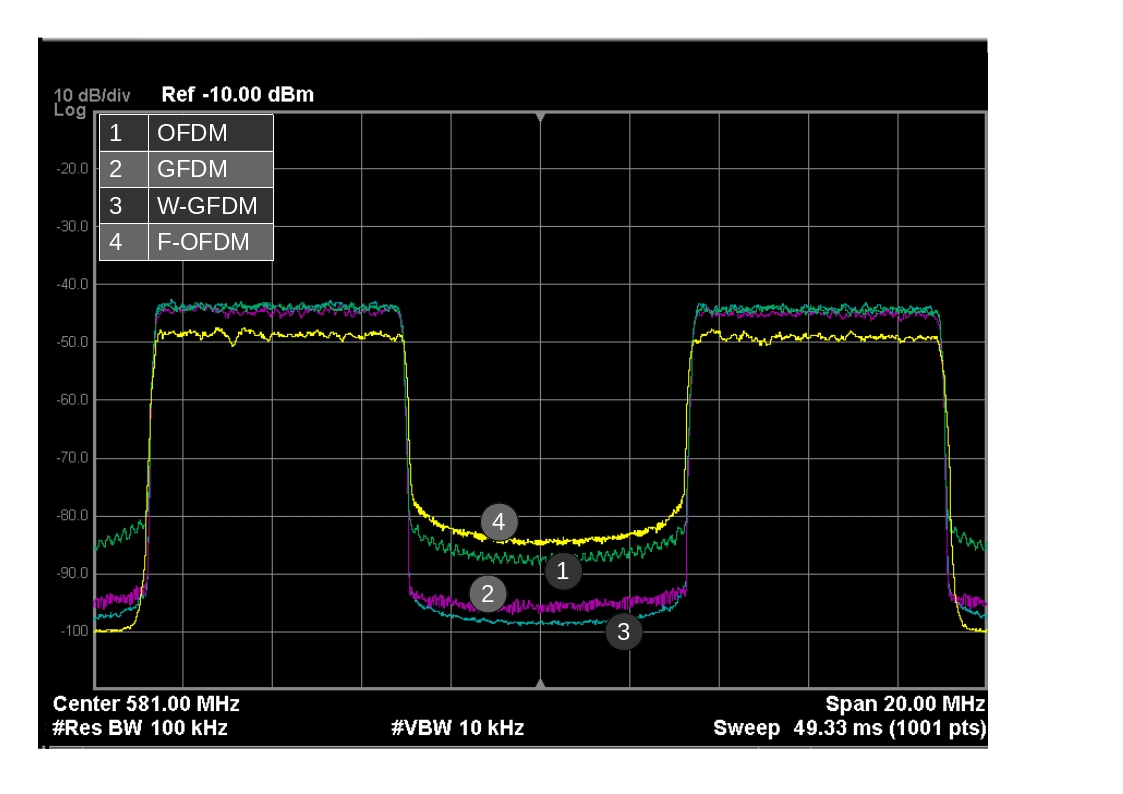
\includegraphics[width=0.48\textwidth]{Figures/5G_WaveformsCompare.jpg}
    \caption{Waveforms out of band emission comparision}
    \label{fig:waveforms}
\end{figure}
%/ 07 Conclusion: 
Section {Conclusions}
%========================================================
The objective of this paper was to purpose a method of test procedure and evaluate the coexistence of different technologies ...
that are candidates for the next generation of mobile communications,  operating in an opportunistic way in the spectrum in coexistence with the Brazilian standard of digital TV ISDB-T. Couple

5G WRAN 
%=========================================================
Though a small number of ISDB-T receivers were used, it was/ is affirmed that there are considerable variations between the reception thresholds according to the receptor model.
The tests presented in this article demonstrate that transmission techniques proposed for 5G as GFDM janellated and F-OFDM have advantages when considering the emission for the range and fragmented use of the spectrum. From these values one can estimate what would be the limitations in the characteristics of operation or installation of systems transmitting in secondary character. Couple

%=======================================================
This work aims to assist in the survey of protection relations, to determine the emission masks that allow 5G systems to coexist with the existing products systems. Couple

%//========================================== 
\bibliographystyle{IEEEtran}
\bibliography{references}

\end{document}
